\section{Results}
\label{sec:results}

\subsection{BTS with two possible power states}
\label{subsec:results1}
The following results were obtained through simulation experiments driven by real traffic traces and deployment geography. The experiments perform a combination of activation of BTS power-saving mode on BTSs alongwith a periodic update of serving BTS for each active call, such that the instantaneous energy consumption in the network is minimized.

First, we consider the benefit of BTS power-saving alone, resulting from traffic diversity at each BTS compared to running the network in the default configuration. The percentage reduction in energy consumption is listed in table~\ref{tab:psonly}. The results indicate that a saving of between 4\% and 12\% can be achieved in a network just by activating BTS power savings. We note here that some of these results are in agreement with Ericsson's claim of saving 10-20\% energy by using BTS power-saving on Germany's Vodafone network~\cite{ericssonclaim}. 

In absolute terms, this represents a cumulative saving of between 43 kWh and 217 kWh per day on 26 BTSs. Now, consider that there are five cellular oeprators in Pakistan: Mobilink with more than 8500 sites~\cite{mobilinksitecount}, Ufone with more than 8000 sites~\cite{ptaannreport}, Zong with more than 5500 sites~\cite{ptaannreport}, Telenor with more than 7000 sites~\cite{telenorsitecount} and Warid with more than 4500 sites~\cite{ptaannreport}. Overall, there were more than 31000 sites in Pakistan at the end of 2011. We extrapolated the daily energy savings number over 26 BTSs to calculate the daily energy savings possible for a country like Pakistan with over 31000 BTSs (see the last row of table~\ref{tab:psonly}). The results indicate that mere activation of BTS power saving option itself can save quite a bit of electrical energy, a critical resource, especially in a developing country. As we shall see next, greater energy savings are possible if we couple periodical call shuffling with BTS power savings in the network. 

\begin{table}
\centering
\begin{tabular}{|c|c|c|c|}
\hline Energy saving & Model 1 & Model 2 & Model 3 \\
\hline Percentage & 4.73\% & 5.43\% & 12.89\% \\
\hline Daily absolute saving & 43.28 & 109.68 & 217.12 \\
over 26 BTSs (in kWh) & \ & \ & \ \\
\hline Country-wide daily saving & 51.6 & 130.77 & 258.87\\
over 31000 sites (in MWh) & \ & \ & \ \\
\hline
\end{tabular}
\caption{Energy savings by using BTS power savings only}
\label{tab:psonly}
\end{table}


If periodic optimization of call placement is coupled with BTS power-saving, the energy saving improves, as shown in Figure~\ref{fig:results2}.
%As noted earlier, we expect to achieve greater energy savings by periodically handing-off calls from busier BTSs to nearby BTSs with lower traffic to put a maximal number of BTSs in power-saving mode. If the periodic re-optimization is done aggressively, the network would remain in a nearly optimal state more often. On the other hand, a less aggressive policy would have the network in a nearly optimal state less often. We, therefore, expect that savings in power consumption should increase when the interval between re-optimization episodes is decreased. Since we are interested in the overall impact of the power saving scheme, the percentage power savings are computed over the entire network and not per BTS. %Furthermore, the percentage savings are computed over the default mapping of calls to BTSs, i.e., each call is associated with the BTS that the caller receives the strongest radio signal from.
%
%The percentage reduction achieved by using Low-Carb for the three BTS models is plotted in Figure~\ref{fig:results2}. 
For all three BTS models, we see an almost linear increase in power saving as the duration of the re-optimization interval is decreased. Recall that the three models are significantly different in terms of power consumption (see Table~\ref{tab:models}). We can not directly say that because model 3 BTS offers the highest percentage reduction in energy consumption, it also saves the most energy (in kWh). %The results in Figure~\ref{fig:results2} are quite useful to study the sensitivity of Low-Carb to the duration of re-optimization interval. However, one can't compare the three BTS models based on that, because the power consumption profiles are different for the three. For instance, a $15\%$ saving on $100kWh$ is not the same as a $15\%$ power saving on $500kWh$.

%\begin{figure}
%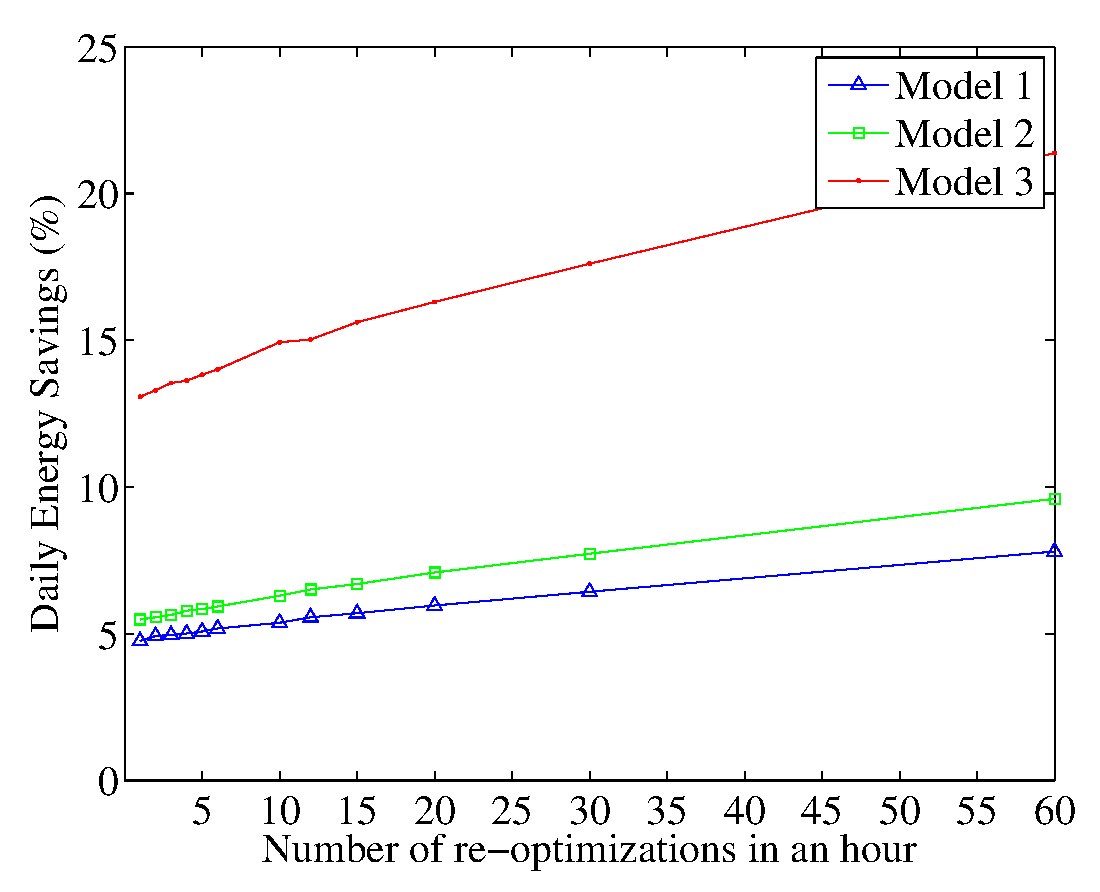
\includegraphics[width=0.5\textwidth]{figures/percent.savings.powersaving.eps}
%\caption{Percentage reduction in power consumption vs re-optimization interval - BTS Power Saving only}
%\label{fig:results1}
%\end{figure}

\begin{figure}
\centering
\subfigure[]{
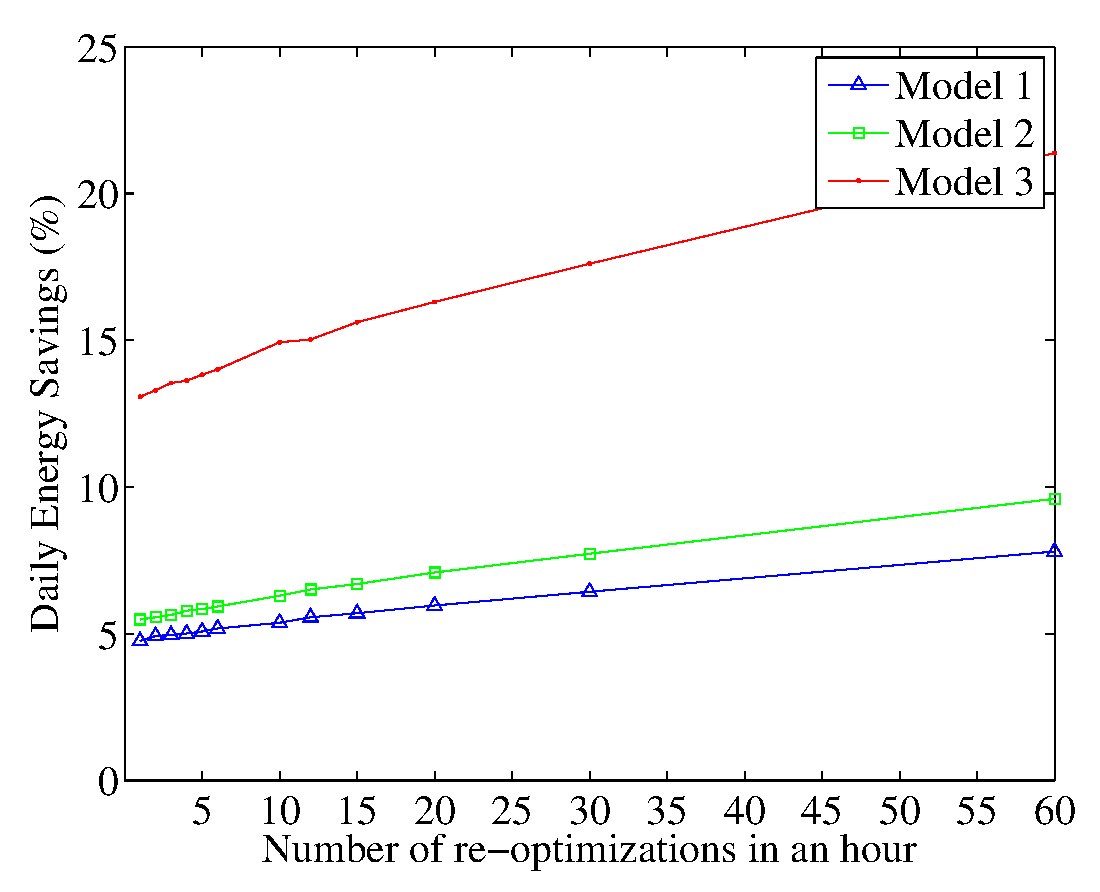
\includegraphics[width=0.45\textwidth]{figures/percent.savings.powersaving.eps}
\label{fig:results2}
}
\subfigure[]{
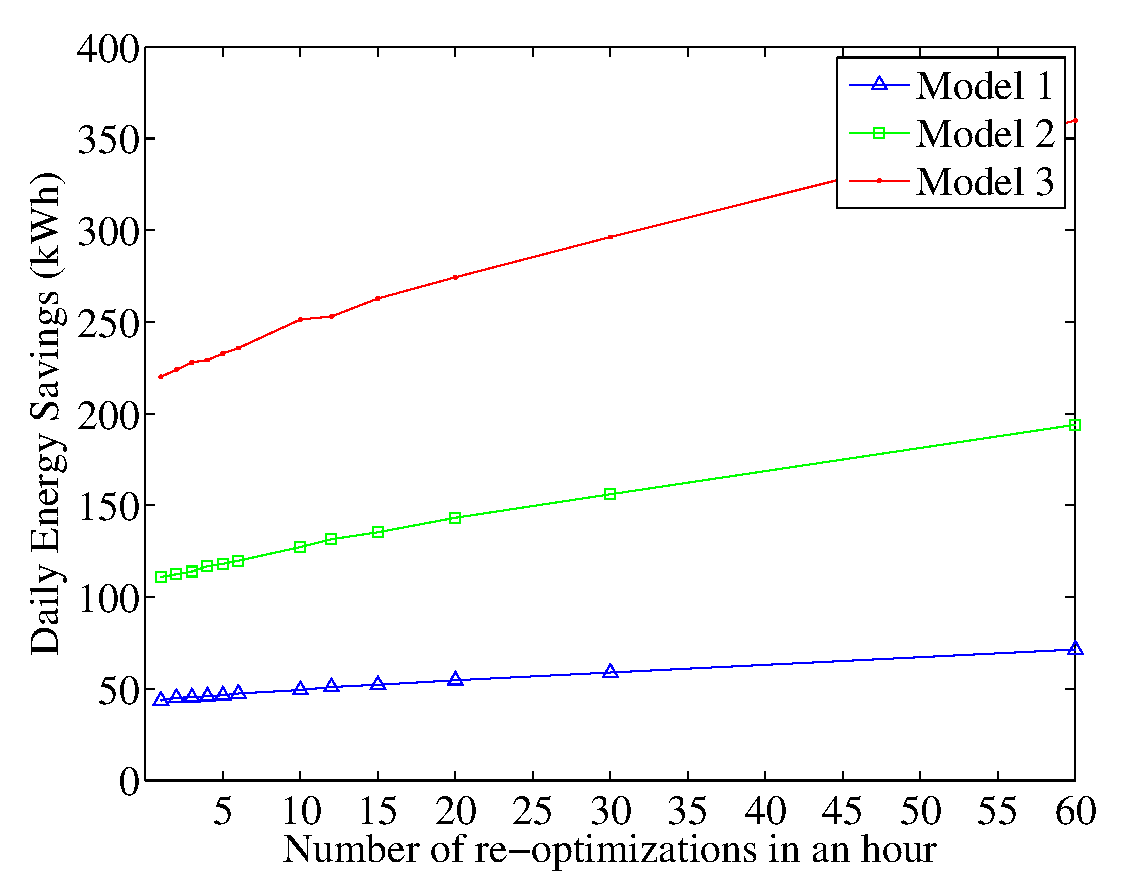
\includegraphics[width=0.45\textwidth]{figures/e.savings.powersaving.eps}
\label{fig:results4}
}
\caption{(a) Percent reduction in energy consumption vs re-optimization interval, (b) Reduction in energy consumption vs re-optimization interval} 
\label{fig:results24}
\end{figure}


%\begin{figure}
%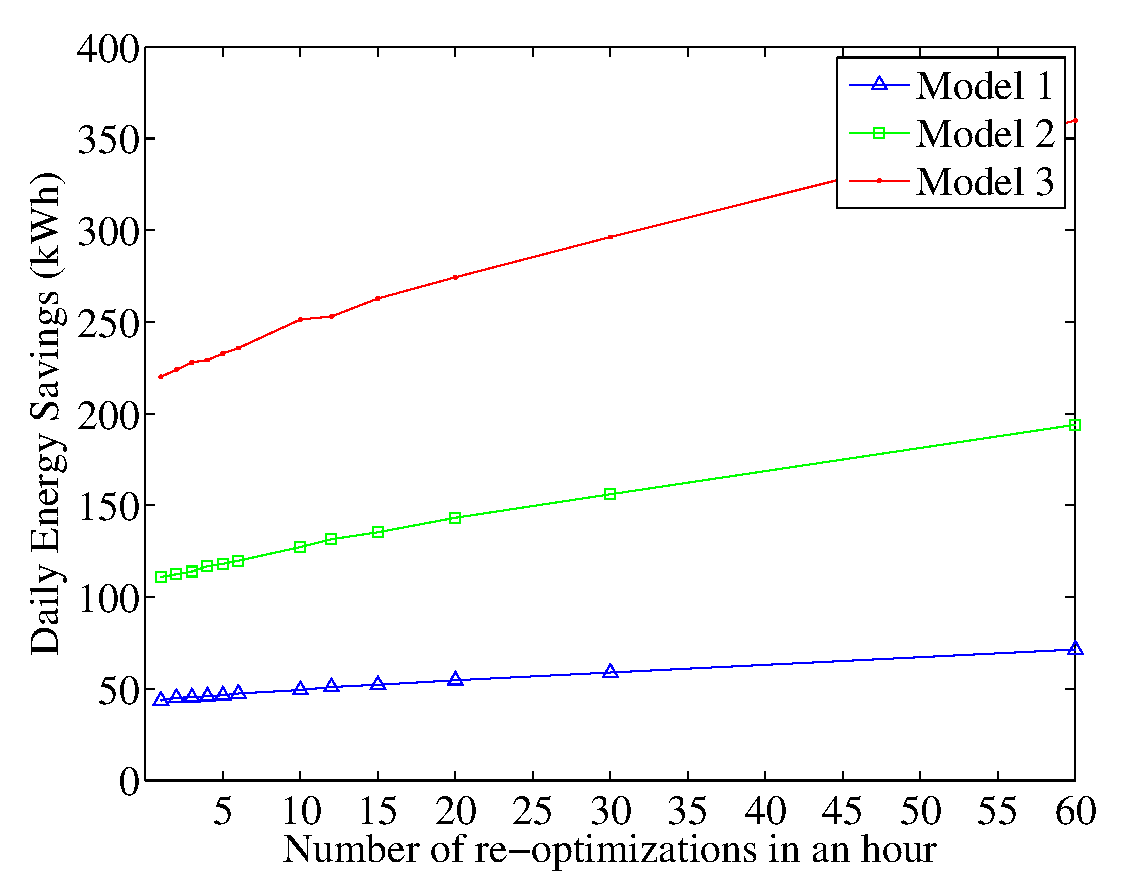
\includegraphics[width=0.5\textwidth]{figures/e.savings.powersaving.eps}
%\caption{Reduction in energy consumption through BTS Power Saving}
%\label{fig:results3}
%\end{figure}

To \textit{compare} the three BTS models in terms of energy saving potential, we also present the absolute reduction in energy consumption for the three BTS models in Figure~\ref{fig:results4}. We see the same linear trend alongwith the same relative order of the three models in terms of amount of saved energy, as in Figure~\ref{fig:results2}. 

Re-optimizing at an interval less than the mean call duration should offer greater savings than a less frequent re-optimization, because the former regime has the opportunity to optimize more by handing off most of the calls. This is confirmed in our results. For instance, for model 1 BTS, the gain in energy savings going from a 60 minutes inter-optimization interval to 30 minutes gains an energy saving of only 0.0506 kWh per minute, while decreasing the inter-optimization interval from 2 minutes to 1 minute gains 12.5421 kWh. %We notice a more pronounced separation between the three models in Figure~\ref{fig:results4}, resulting from the considerable difference between the maximum and minimum power consumption levels for the three models, as well as the values of $\gamma$.

Let us now interpret what these results mean physically in terms of ecological impact. If we extrapolate our results, the total energy saving for Pakistan are projected to be $60.72$ MWh, $156.84$ MWh and $301.61$ MWh daily, respectively, according to the three BTS models. These savings in energy are significant, especially for small and developing countries. Since network deployments and traffic patterns are similar in different countries, we also expect that similar savings should be achievable in many other countries as well.

In the above extrapolation, we have assumed that the same amount of energy saving would be applicable in rural as well as urban settings. While this may not necessarily be true because the deployments are sparse in rural settings, resulting in reduced potential to save energy by means of call hand-off to neighboring sites, the potential to save energy merely by BTS power-saving should be higher in a rural setting because traffic loads are typically lower.

\subsection{Multi-state BTS}
\label{subsec:results2}
In our experimental results discussed so far, we have observed that going from a 6+6+6 configuration to a 2+2+2 configuration can save a significant amount of energy. Intuition suggests that going to a finer granularity of resource pruning should enable greater energy savings. We now present two cases that are different from the configuration considered so far. In the first case, we consider the ability to (de)activate TRXs in pairs, i.e., a site may be in one of three configurations at a given time: 6+6+6, 4+4+4 or 2+2+2. In the second case, we consider the ability to (de)activate each TRX on a site independently, i.e., at a given time, a site may be in one of six possible configurations. 

In this scenario, we conducted simulation experiments where a re-optimization was performed every six minutes using model 1 BTS. The results of these experiments are given in Table~\ref{tab:granularityresults}. For all three BTS models, we see that going from a 2-state model to a 3-state model gives a relatively small increase in energy savings compared to the jump from 3-state to 6-state model.  

\begin{table}
\centering
\begin{tabular}{|c|c|c|c|}
\hline
Granularity & BTS Model 1 & BTS Model 2 & BTS Model 3\\
\hline 2-State & 5.38\% & 6.29\% &  14.94\% \\
\hline 3-State & 6.81\% & 7.73\% &  18.62\% \\
\hline 6-State & 14.69\% & 25.33\% &  33.69\% \\
\hline
\end{tabular}
\caption{Percentage electricity savings for different granularity of resource pruning}
\label{tab:granularityresults}
\end{table}

\subsection{Performance of heuristic algorithms}
\label{subsec:heur1-results}
\begin{figure}
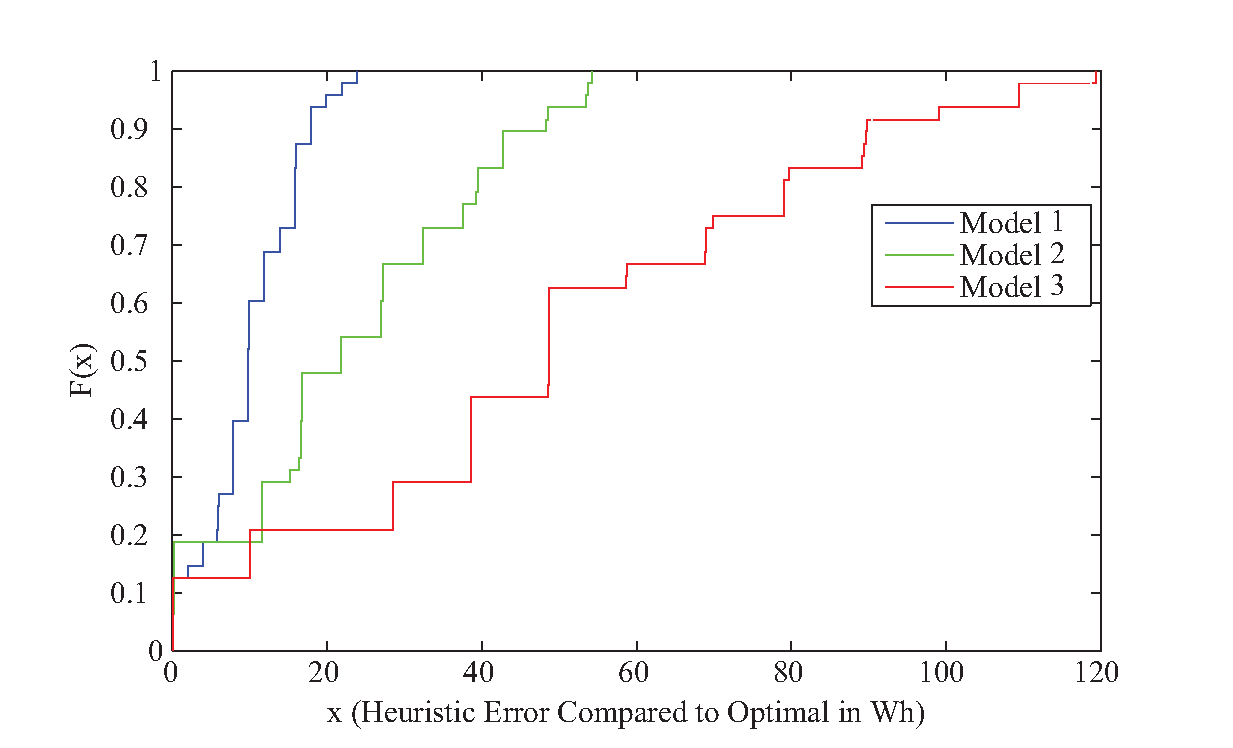
\includegraphics[width=0.5\textwidth]{figures/heuristicerror-touchedup.eps}
\caption{Empirical CDF of the difference between the cost offered by our heuristic compared to the optimal}
\label{fig:results5}
\end{figure}

We also ran experiments for each BTS model in which the electricity cost for the optimal as well as the heuristic algorithms (Algorithm 1 and 2) was computed. We assessed the performance of our heuristics by computing the difference (error) in the electricity cost of the two solutions. For statistical significance, we computed the error in our heuristic relative to the optimal solution over 48 different experiment runs for each BTS model. The resulting CDF of the heuristic error (in Wh) is plotted in Fig.~\ref{fig:results5}. We can see in Fig.~\ref{fig:results5} that our heuristic algorithm 1 is quite close to the optimal solution most of the time, especially for the Model 1 and Model 2 BTS. For Model 3 BTS, although the error is comparatively larger, but since the amount of savings with the optimal solution is quite high (Fig.~\ref{fig:results2}), the heuristic will still result in significant energy savings.  

\subsection{Sensitivity to the value of $\epsilon$}
\label{subsec:results3}
If the value of $\epsilon$ in our optimization is set too aggressively, a BTS that is placed in low-power mode may have to be moved back to high-power mode soon afterwards due to short time scale variations in call volume. Theoretically, it is even possible that there may be several such back and forth transitions at a BTS. Such rapid state oscillations may be undesirable and to avoid these, the value of $\epsilon$ must be set at a safe value. Furthermore, if $\epsilon$ is set too aggressively, a BTS placed in low-power mode would be operating very close to it's \textit{new} and lower traffic capacity. If several calls arrive in a short time window, the BSC may not have sufficient time to bring the BTS back into high-power mode and, thus, some calls may be blocked. However, if $\epsilon$ is set too conservatively, the energy savings would be smaller. 

We carried out experiments to assess the impact of the value of $\epsilon$ on the energy savings achievable through RED-BL. For this purpose, we fixed the inter-optimization interval at 6 minutes and carried out RED-BL optimizations for all three BTS models. Furthermore, we considered a two-state BTS model, i.e., a BTS may be placed in either a 6+6+6 or a 2+2+2 configuration. The range of possible values for epsilon were 5, 10, 15 and 25. Since the traffic capacity of a 2+2+2 BTS is 44\footnote{The capacity of the 2+2+2 BTS is 3$\times$2$\times$8 = 48, but 4 channels were reserved by the operator for control and broadcast channels.}, any larger value for $\epsilon$ did not make sense. Figure~\ref{fig:case2:results6} shows the results. As expected, the percentage savings deplete almost linearly with increasing values of $\epsilon$.

\begin{figure}
\centering
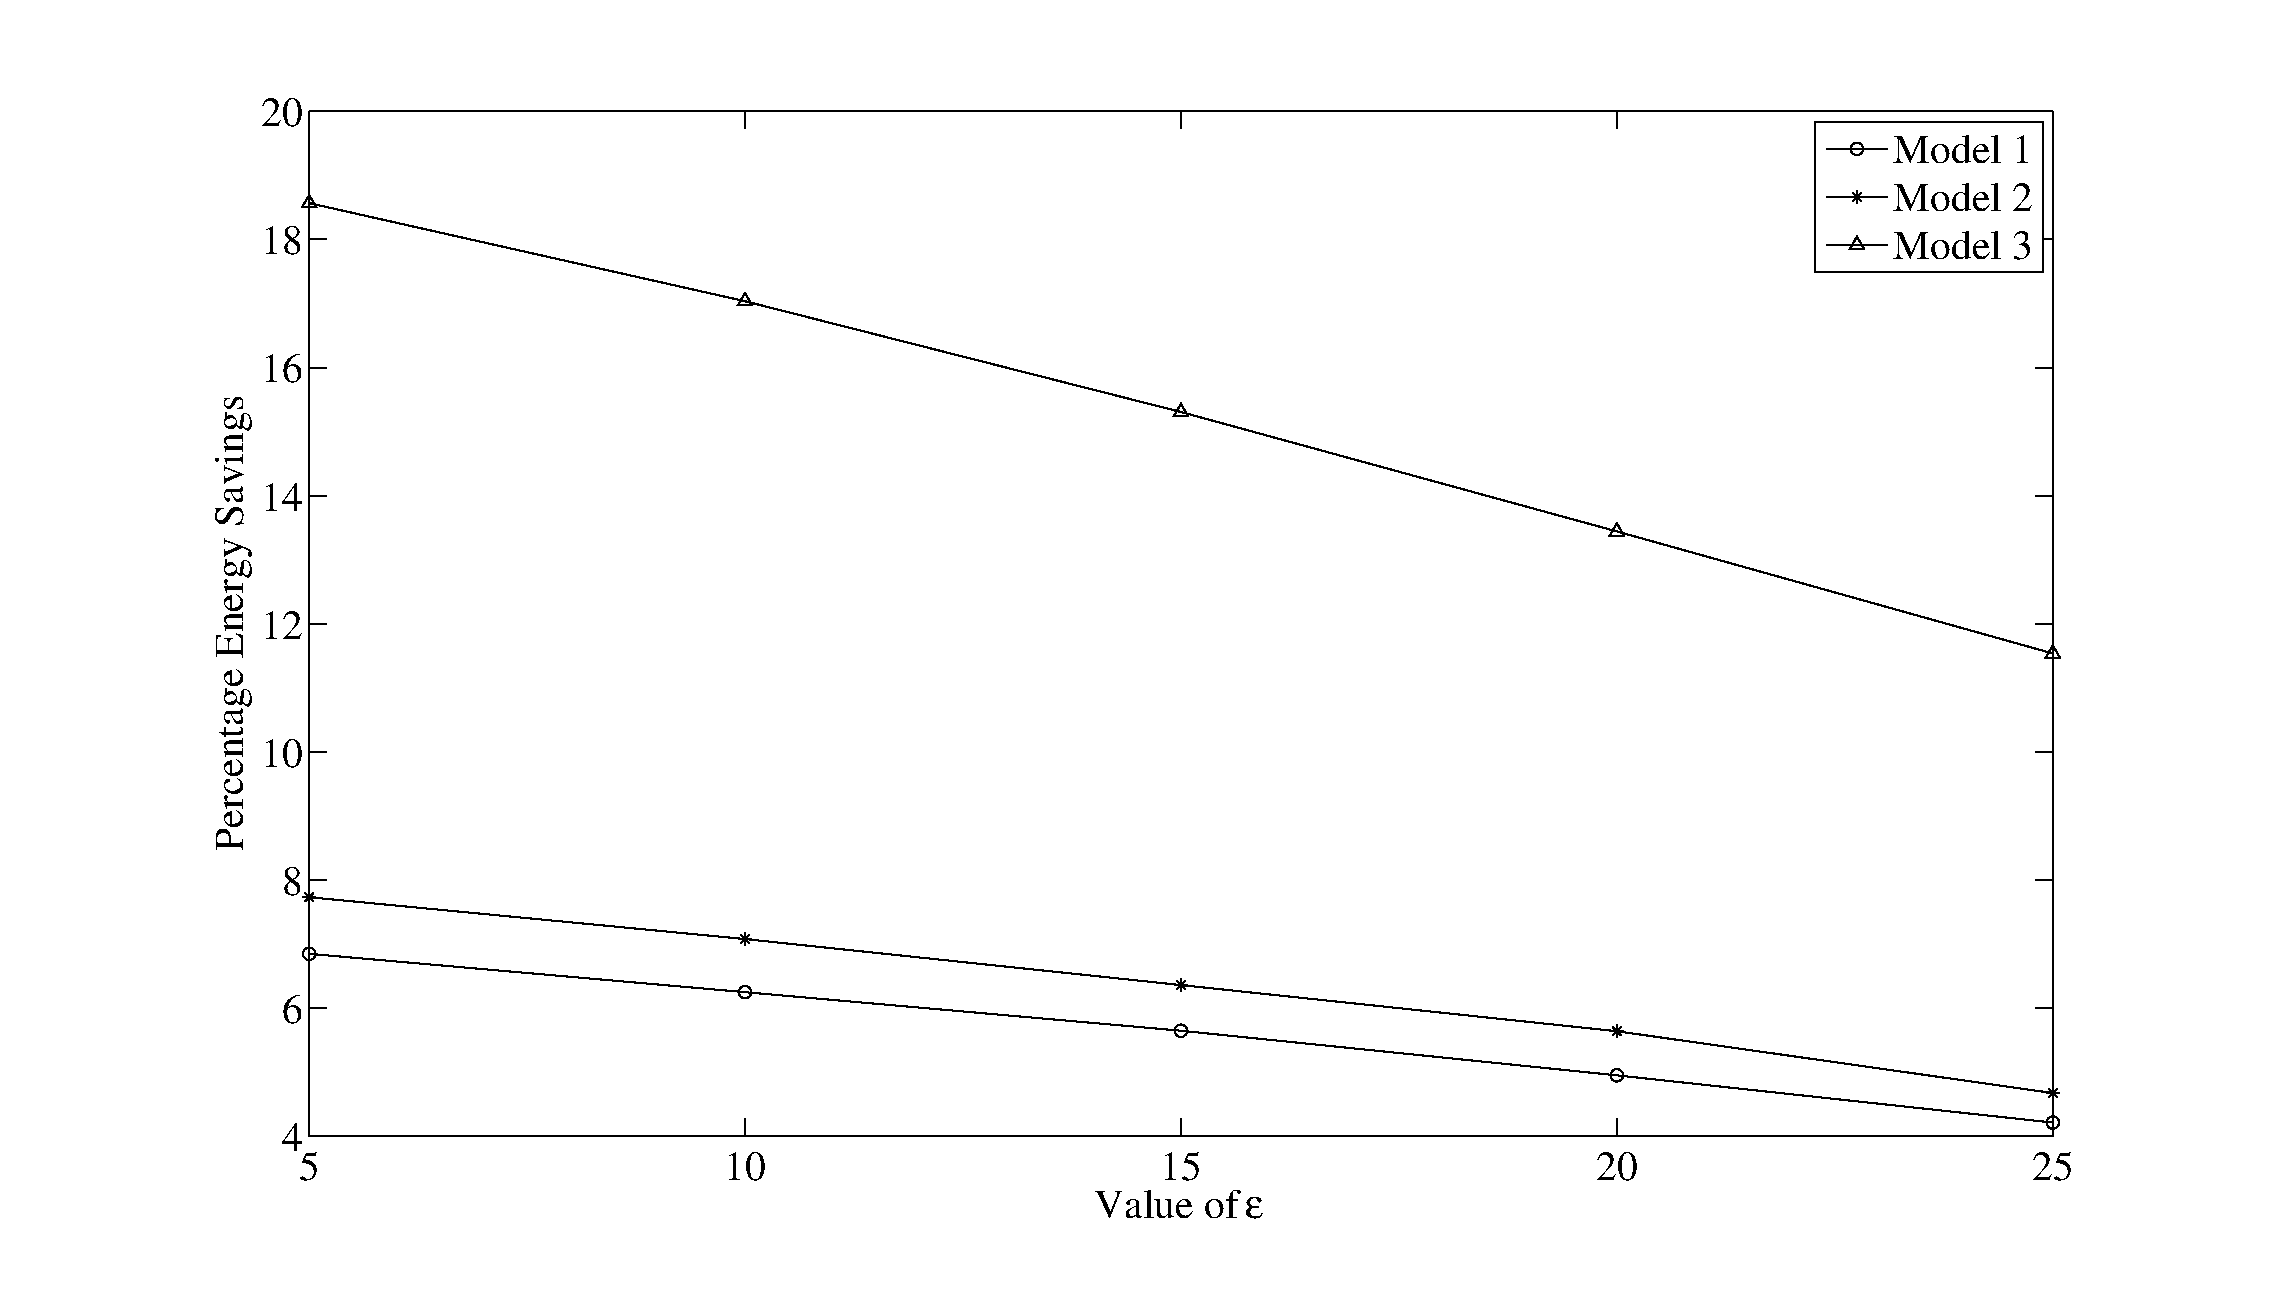
\includegraphics[width=0.8\textwidth]{figures/epsilonresults.eps}
\caption{The percentage energy savings for all three BTS models considered in this paper vs the value of $\epsilon$, with a six minute inter-optimization interval}
\label{fig:case2:results6}
\end{figure}

%\subsection{Discussion}
%\label{subsec:discuss:case2} 
%Through simulation experiments, we have seen that Low-Carb may cut electricity costs for cellular operators and save large amounts of electrical energy. Low-Carb

%An assumption in the above extrapolation is that the same amount of energy can be saved anywhere in the network. However, traffic patterns and deployment denisty vary in a given network. For instance, cellular networks in rural areas are typically characterized by lower traffic alongwith sparse deployments and, therefore, may not offer as much energy saving possibility as an urban setting (our dataset is for an urban setting). We do not expect that there would be no opportunity for energy savings in rural settings, because of multiple factors. This is partially correct because saving more energy by call-handoff is tough due to sparse deployments. However, the traffic is typically low in such areas, so there should be a greater opportunity to deactivate TRXs most of the time, resulting in greater savings in rural areas than urban. In an extended version of this paper, we will experiment with a dataset from a live network in a rural setting to assess the overall savings possible in a country-wide network.

%\begin{figure}
%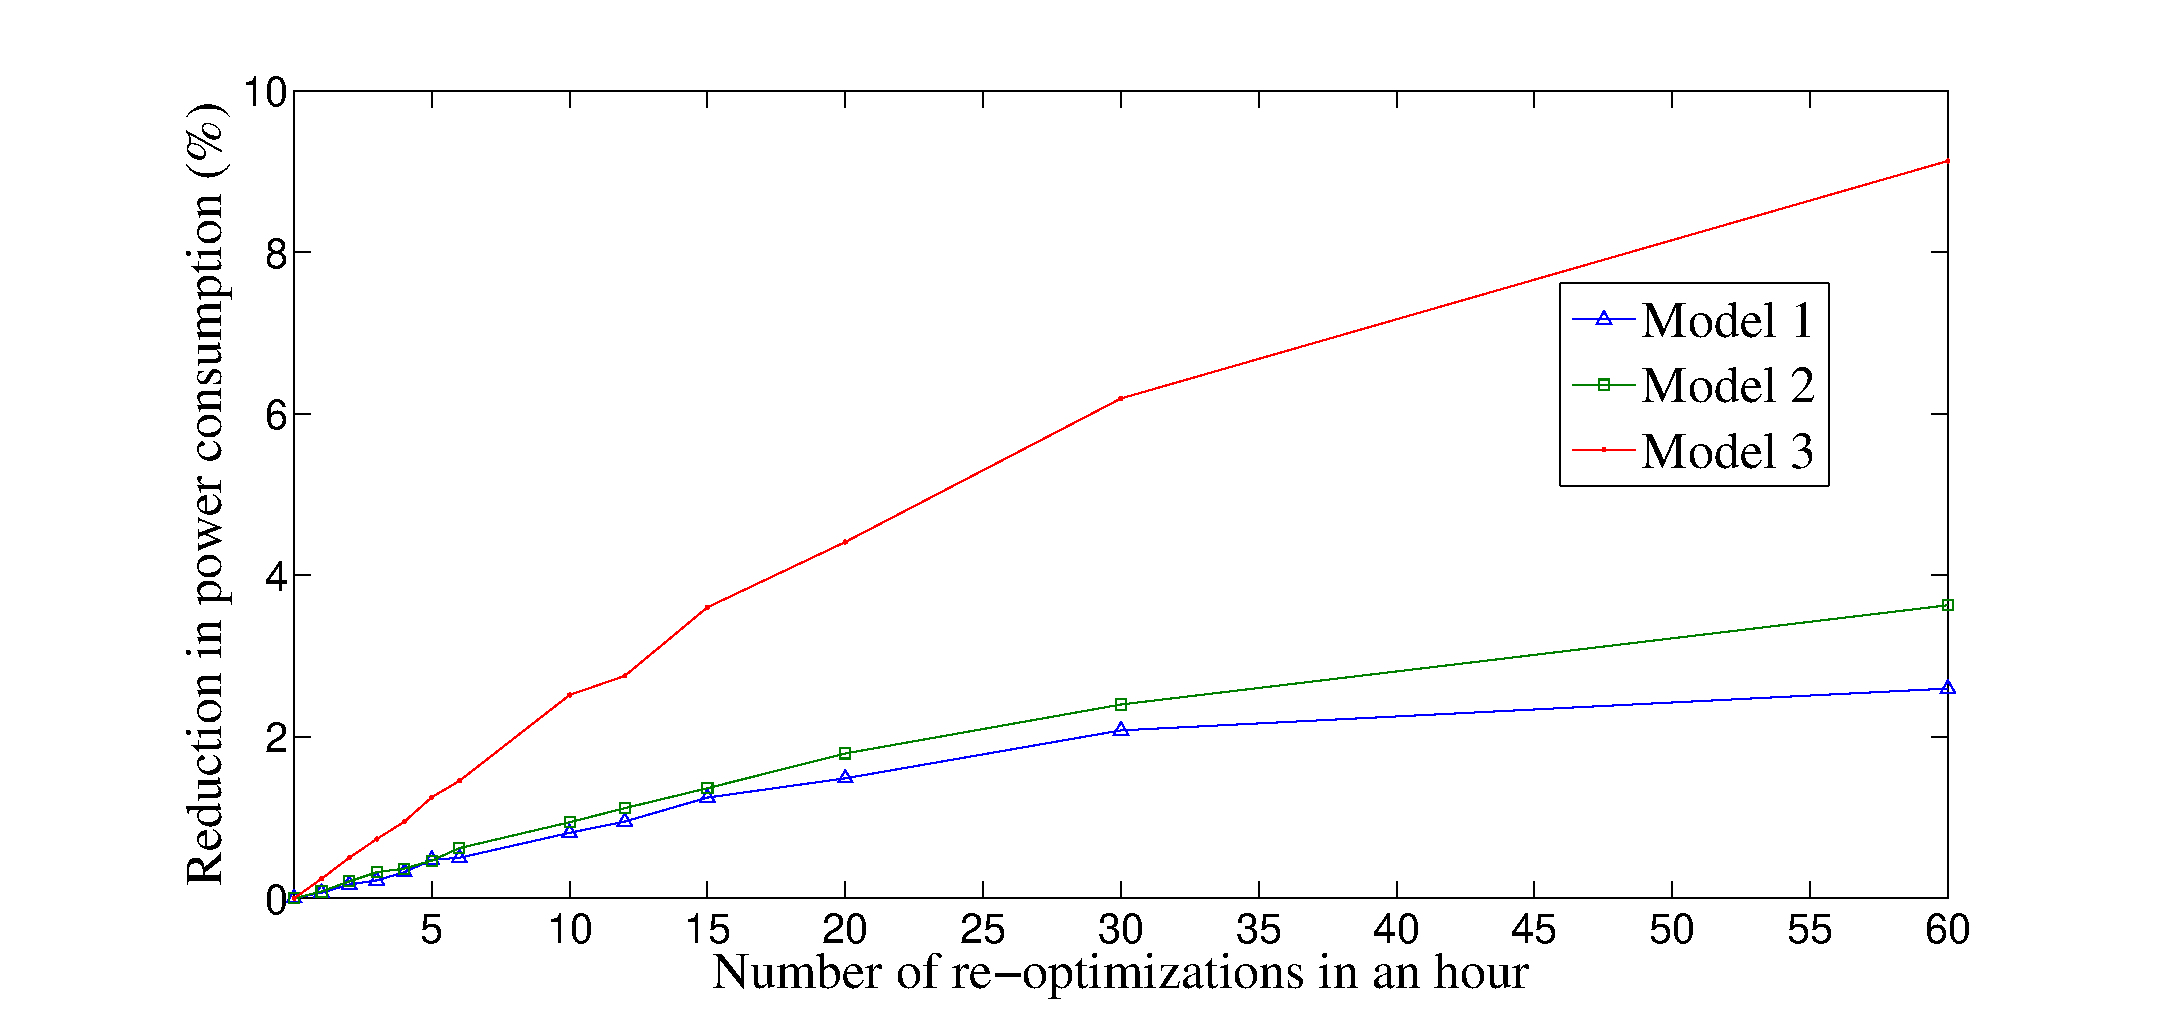
\includegraphics[width=0.5\textwidth]{figures/improvementplot.eps}
%\caption{Percentage reduction in power consumption vs re-optimization interval - Sparse deployment of $9$ BTSs}
%\label{fig:results1}
%\end{figure}
%
%For a region with sparse deployments, we plot the percentage savings in power consumption as the re-optimization interval was varied, in Figure~\ref{fig:results1}. For model 1 BTS, we were only able to reduce the power consumption by about $2.5\%$ even if we re-optimized once every minute. This is expected because placing a BTS in power saving mode affords a saving of $240W$ (the value of $\gamma$), which is a small percentage of the maximum power consumption($1500W$) and this small saving is applicable only while the traffic at a BTS is below $\delta$.
%
%The percentage savings for model 2 BTS are somewhat better than those for the model 1 BTS. This would be due to the value of  $\gamma$ being a larger fraction of the overall site power consumption than model 1. For model 3 BTS, the value of $\gamma$ is a pretty large fraction of the overall site configuration, so as expected, we see larger overall percentage reduction in power consumption.
%
%A comparison of energy savings for the three BTS types using percentage energy savings does not give the whole picture because the overall power consumption of the three types are different. To put the savings in perspective, we plot the amount of energy (kWh) saved per day over $9$ BTSs, using the proposed scheme. For the sparse deployment, the results are plotted in Figure~\ref{fig:results2}.
% 
%\begin{figure}
%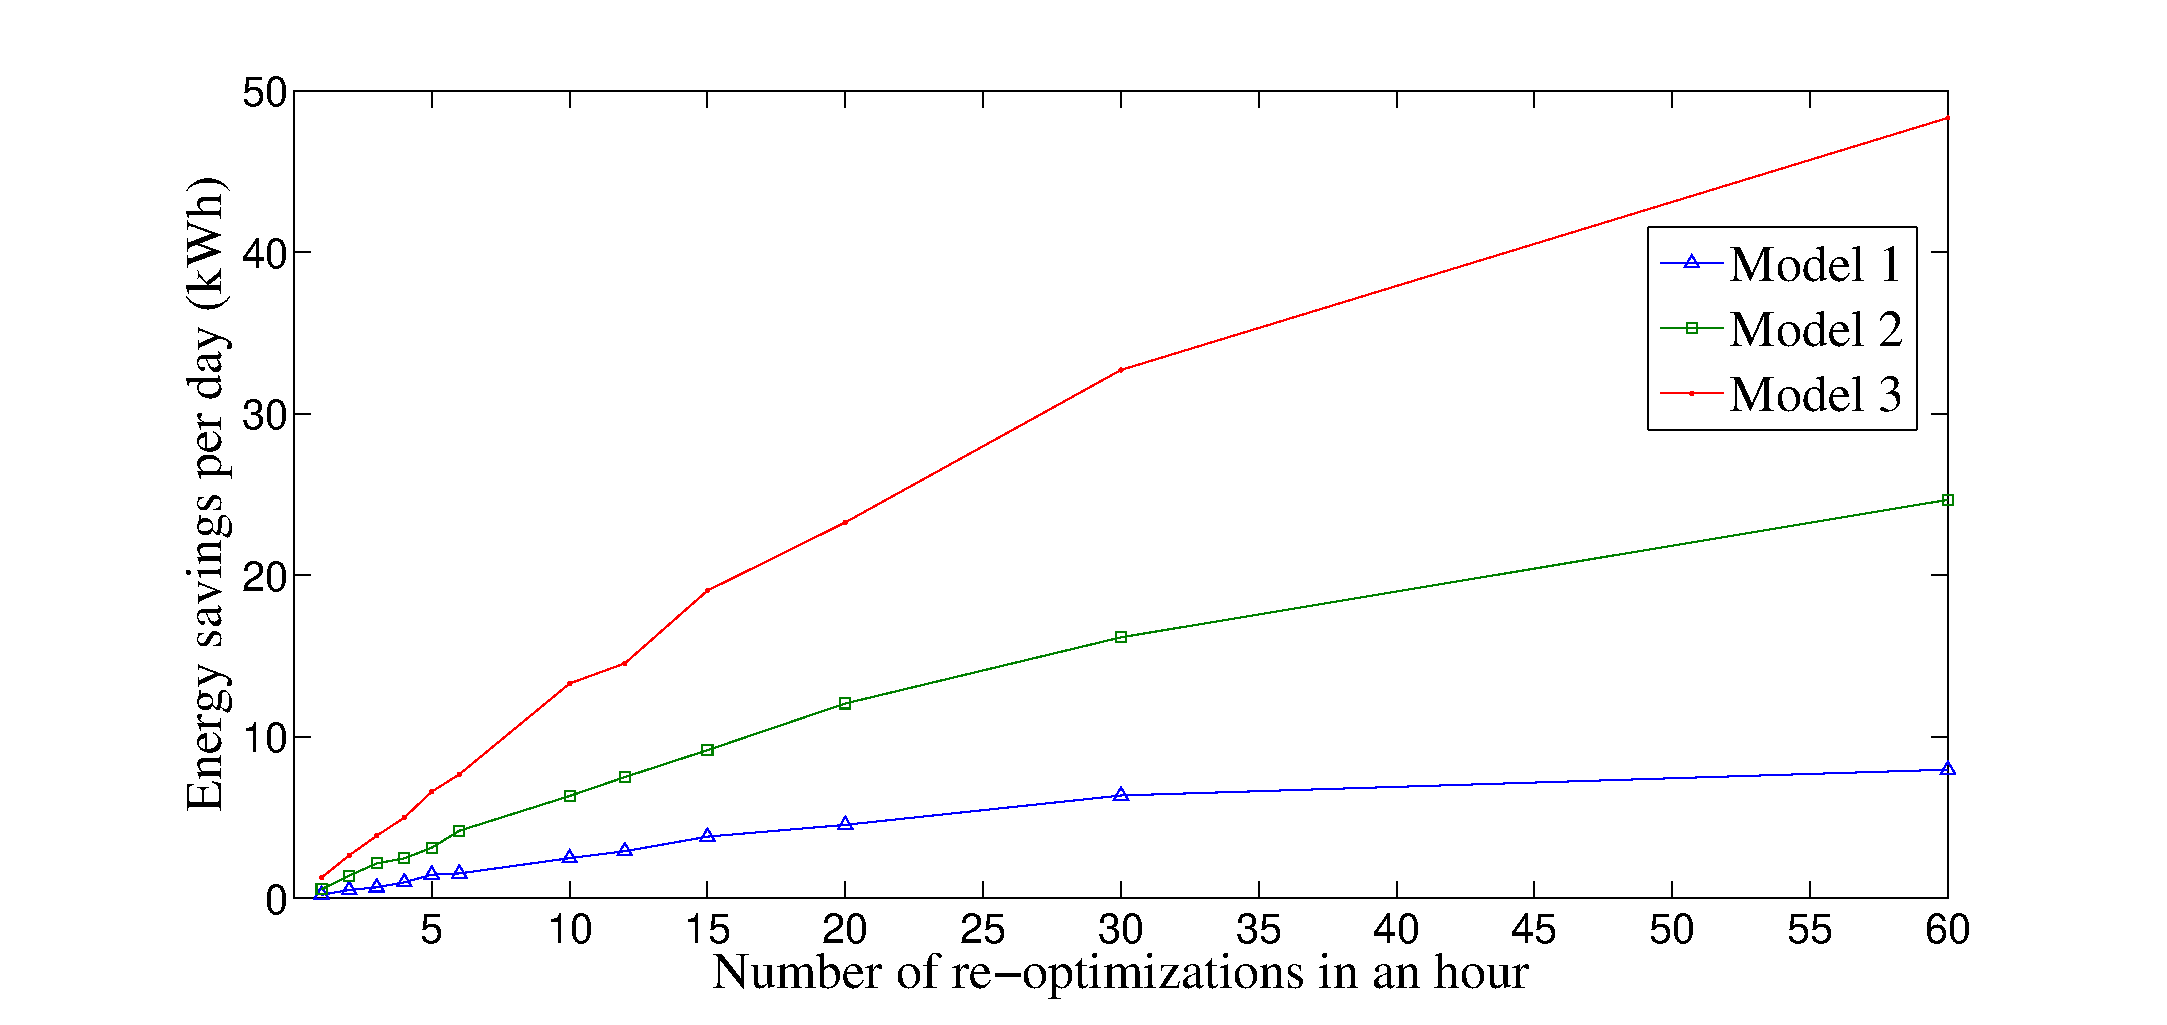
\includegraphics[width=0.5\textwidth]{figures/energysavingssparse.eps}
%\caption{Amount of energy saved per day (kWh) - Sparse deployment of $9$ BTSs}
%\label{fig:results2}
%\end{figure}
%
%We can see the same pattern in the amount of energy saved for the three models as we did for the percentage reduction in power consumption, albeit with model 2 differentiating itself somewhat more clearly from model 1. This is clearly because there is a large difference between the maximum power consumption for model 1 and 2.
%
%One can see in Figure~\ref{fig:results2} that when re-optimization is done every $5$ minutes, one may be able to save approximately $2.5kWh$, $7kWh$ and $15kWh$ respectively with model 1, 2 and 3. This saving is achieved over a set of $9$ BTSs. In order to understand what kind of savings this translates into for an operator in a country like Pakistan, consider that for an operator named Telenor that has over $7000$ sites in Pakistan~\cite{telenorsitecount} $1800MHz$ band, our results approximate a daily saving of $105MWh$.
%
%For a dense deployment of $9$ BTSs, results of the same set of experiments are plotted in Figure~\ref{fig:results3} and Figure~\ref{fig:results4}. These graphs show the same trends as observed for the sparse deployment but with greater magnitudes. For a dense deployment, for instance, when optimizing every $5$ minutes, the savings afforded in a dense deployment for model 3 were about $10kWh$ per day.
%
%\begin{figure}
%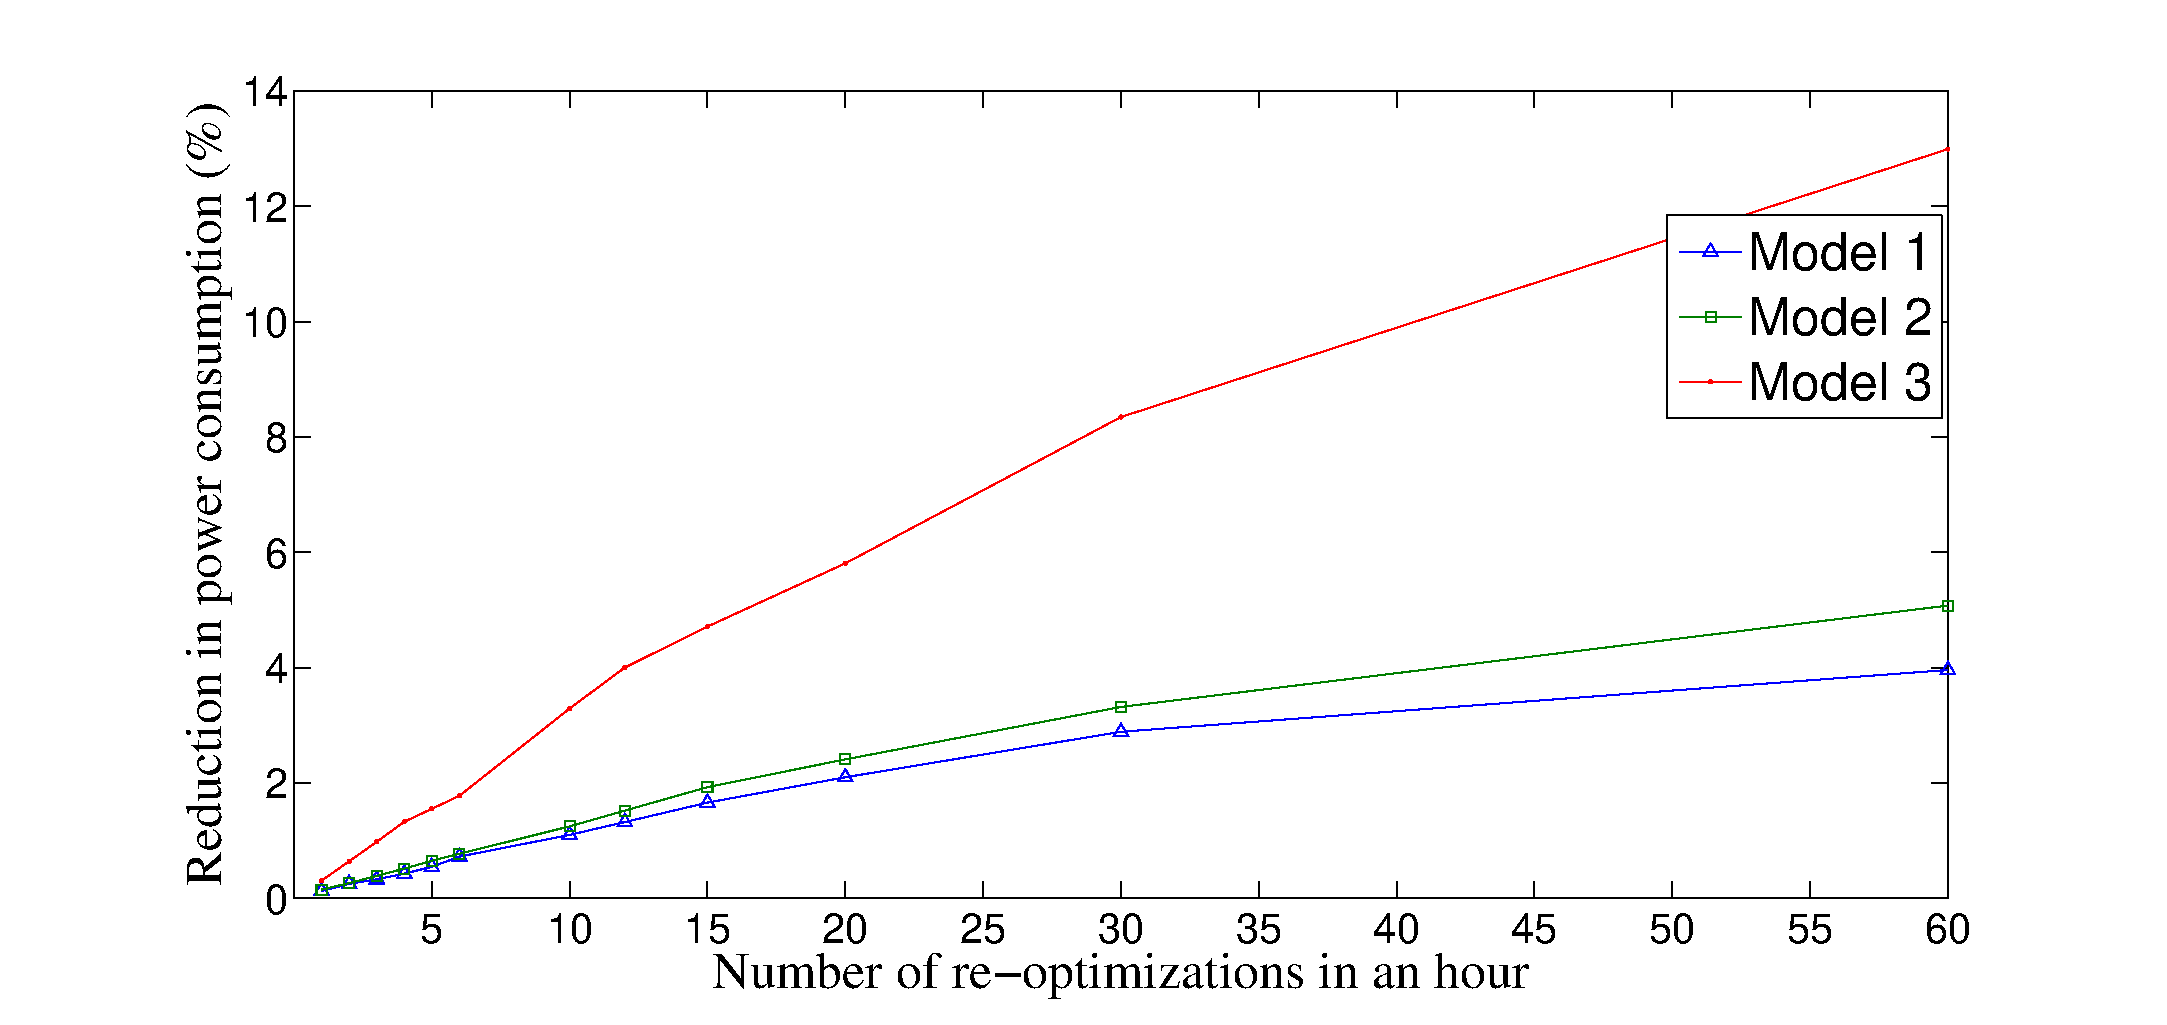
\includegraphics[width=0.5\textwidth]{figures/improvementplotdense.eps}
%\caption{Percentage reduction in power consumption vs re-optimization interval - Dense deployment of $9$ BTSs}
%\label{fig:results3}
%\end{figure}
%
%\begin{figure}
%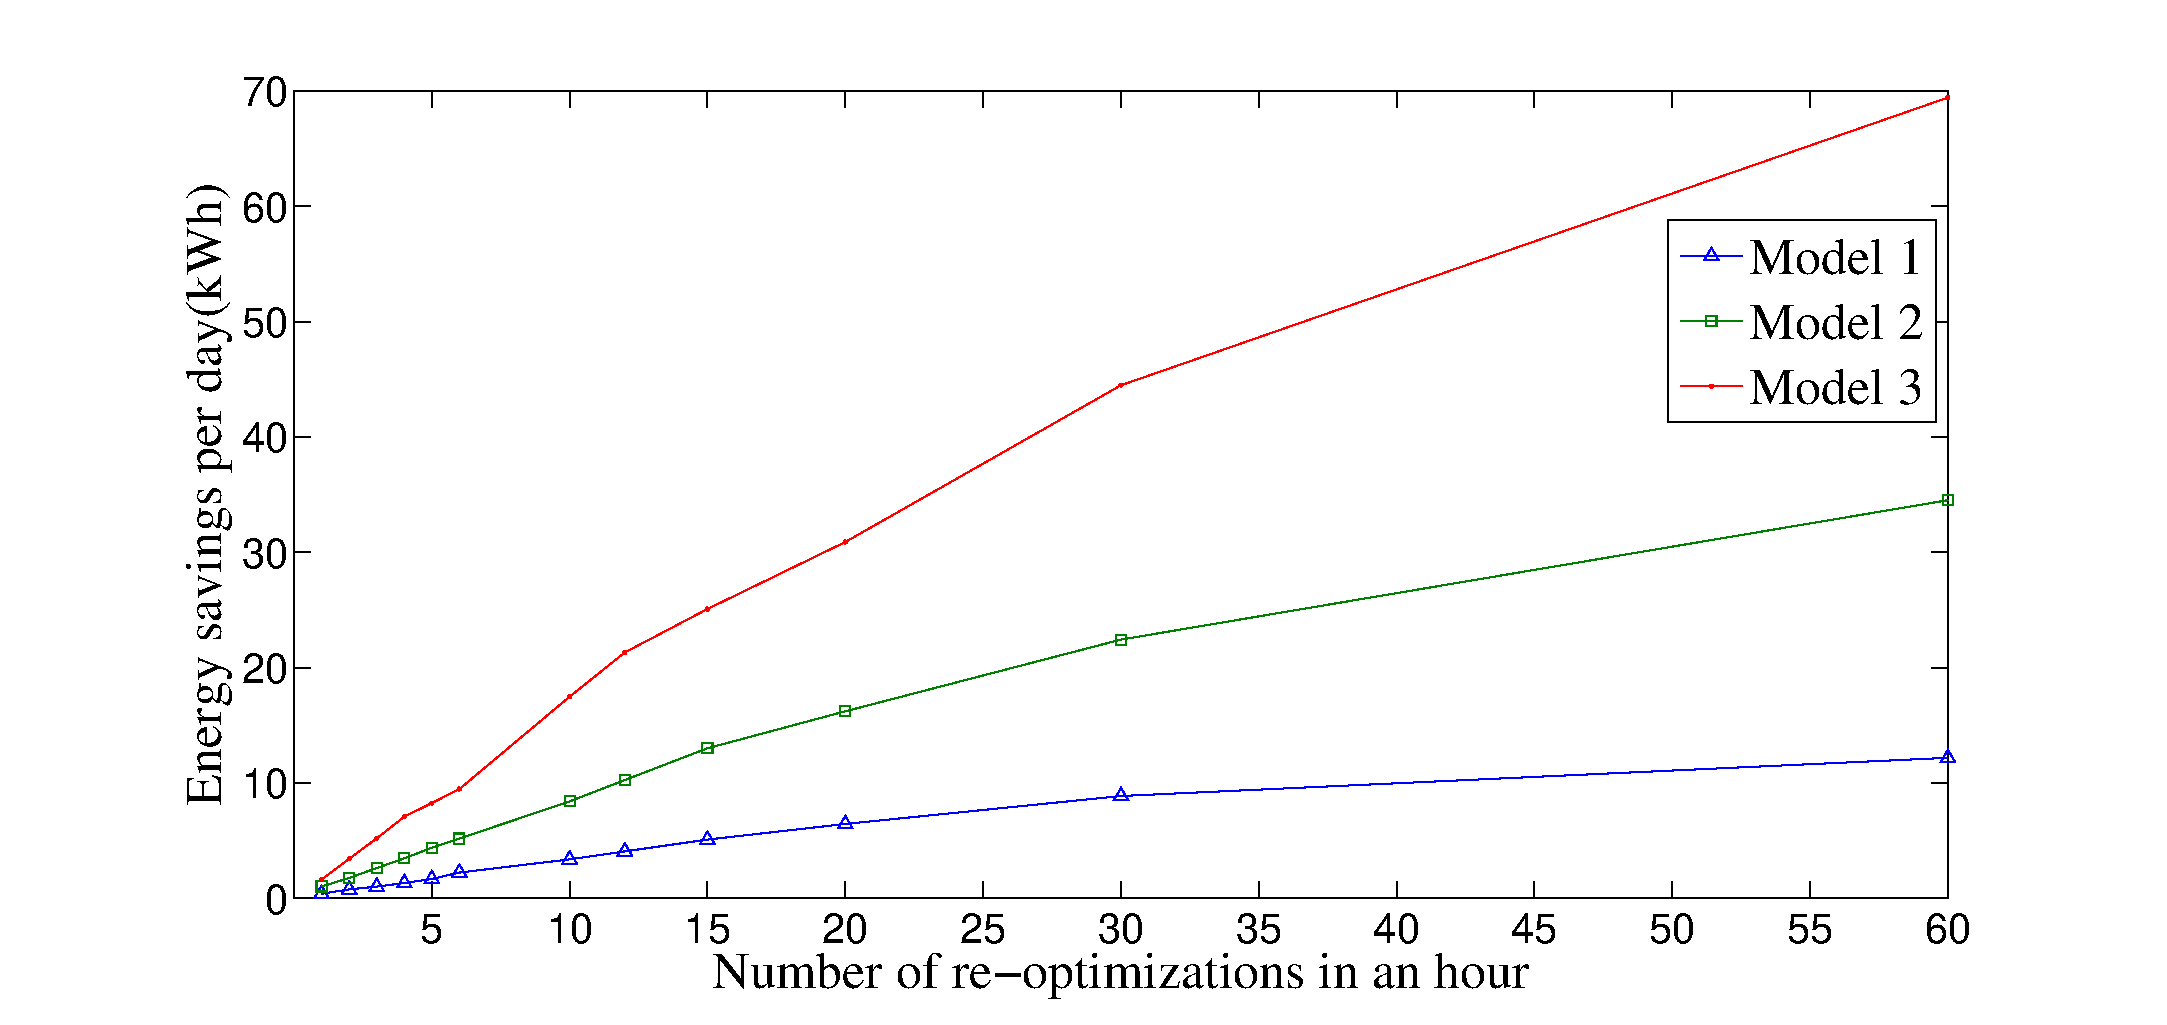
\includegraphics[width=0.5\textwidth]{figures/energysavingsdense.eps}
%\caption{Amount of energy saved per day (kWh) - Dense deployment of $9$ BTSs}
%\label{fig:results4}
%\end{figure}
%
%An operator's network is typically a mix of sparse and dense deployments depending on the spread of subscriber density in their coverage area. For a range of sparse/dense deployment mixes, we computed the approximate achievable reduction in annual energy consumption using the proposed technique. This calculation is just a weighted average of the energy consumption reduction for the sparse and dense deployment as obtained in our experiments. To conserve space, we are listing results only for the case when re-optimization is done every $5$ minutes. The results are listed in table~\ref{tab:benefits}.
%
%\begin{table*}
%\centering
%\begin{tabular}{|c|c|c|c|c|c|c|c|c|c|}
%\hline BTS Model & \multicolumn{9}{|c|}{Sparse/Dense deployment mix (percentages)}\\
%\cline{2-10} \ & 10/90 & 20/80 & 30/70 & 40/60 & 50/50 & 60/40 & 70/30 & 80/20 & 90/10\\
%\hline 1 & 27.58 &	26.77 &	25.97 & 25.16 & 24.35 &	23.55 &	22.74 &	21.94 &	21.13 \\
%\hline 2 & 69.81	& 67.88	& 65.96	& 64.04	& 62.12	& 60.19	& 58.28 & 56.35	& 54.43 \\
%\hline 3 & 144.39 & 139.66	& 134.93	& 130.19	& 125.45	& 120.72	& 115.98	& 111.24	& 106.51
% \\
%\hline
%\end{tabular}
%\caption{Estimated annual energy savings (MWh) for $7000$ sites in \\ various mixes of sparse and dense deployment}
%\label{tab:benefits}
%\end{table*}

%It is important to consider the cost of this scheme if it is to be deployed in practice. On average, each re-optimization took an average of about one minute when run on a laptop computer with a Core i3 processor and 4 GB of RAM, for the 26 BTS dataset that we considered. Further improvements in running time alongwith joint optimization of a greater number of sites simultaneously can be achieved through a more powerful computer and/or parallelization. However, BIP is an NP-Hard problem, so expecting to solve an online optimization of traffic over a city's entire network would be unrealistic. We must, therefore, come up with heuristics to solve this problem sub-optimally. One heuristic, as proposed in this paper is to separately optimize traffic over small sets of BTSs. Other approaches such as approximations to similar classes of problems (such as the assignment problem) and evolutionary algorithms need to be tried and will be explored in an extended version of this paper.